%!TEX root = ../Thesis.tex
\chapter{Appendix}

\subsection{Project code}

The code for the project can be found at:

\url{https://github.com/BiancaDT/ArduinoIMU} 


\subsection{Equations}

%Theta2dotdot

\begin{equation}\label{ddtheta2}
\scalemath{0.3}{\ddot{\theta}{_2} =	
{\frac { \left(  \left( \sin \left( \theta_{{3}} \left( t \right) 
 \right) \sin \left( \theta_{{1}} \left( t \right)  \right) +\cos
 \left( \theta_{{1}} \left( t \right)  \right) \cos \left( \theta_{{3}
} \left( t \right)  \right)  \right)  \left( {\frac {\rm d}{{\rm d}t}}
\theta_{{3}} \left( t \right)  \right) ^{2}+\cos \left( \theta_{{1}}
 \left( t \right)  \right) \sin \left( \theta_{{3}} \left( t \right) 
 \right) -\sin \left( \theta_{{1}} \left( t \right)  \right) \cos
 \left( \theta_{{3}} \left( t \right)  \right)  \right) {\frac {
{\rm d}^{2}}{{\rm d}{t}^{2}}}\theta_{{1}} \left( t \right) + \left( {
\frac {\rm d}{{\rm d}t}}\theta_{{1}} \left( t \right)  \right) ^{2}
 \left(  \left( \cos \left( \theta_{{1}} \left( t \right)  \right) 
\sin \left( \theta_{{3}} \left( t \right)  \right) -\sin \left( \theta
_{{1}} \left( t \right)  \right) \cos \left( \theta_{{3}} \left( t
 \right)  \right)  \right)  \left( {\frac {\rm d}{{\rm d}t}}\theta_{{3
}} \left( t \right)  \right) ^{2}-\sin \left( \theta_{{3}} \left( t
 \right)  \right) \sin \left( \theta_{{1}} \left( t \right)  \right) -
\cos \left( \theta_{{1}} \left( t \right)  \right) \cos \left( \theta_
{{3}} \left( t \right)  \right)  \right) }{ \left(  \left(  4.0\,\cos
 \left( \theta_{{3}} \left( t \right)  \right) \cos \left( \theta_{{2}
} \left( t \right)  \right) + 4.0\,\sin \left( \theta_{{2}} \left( t
 \right)  \right) \sin \left( \theta_{{3}} \left( t \right)  \right) 
 \right)  \left( {\frac {\rm d}{{\rm d}t}}\theta_{{2}} \left( t
 \right)  \right) ^{2}- 4.0\,\sin \left( \theta_{{3}} \left( t
 \right)  \right) \cos \left( \theta_{{2}} \left( t \right)  \right) +
 4.0\,\sin \left( \theta_{{2}} \left( t \right)  \right) \cos \left( 
\theta_{{3}} \left( t \right)  \right)  \right)  \left( {\frac {\rm d}
{{\rm d}t}}\theta_{{3}} \left( t \right)  \right) ^{2}+ \left(  4.0\,
\sin \left( \theta_{{3}} \left( t \right)  \right) \cos \left( \theta_
{{2}} \left( t \right)  \right) - 4.0\,\sin \left( \theta_{{2}}
 \left( t \right)  \right) \cos \left( \theta_{{3}} \left( t \right) 
 \right)  \right)  \left( {\frac {\rm d}{{\rm d}t}}\theta_{{2}}
 \left( t \right)  \right) ^{2}+ 4.0\,\cos \left( \theta_{{3}} \left( 
t \right)  \right) \cos \left( \theta_{{2}} \left( t \right)  \right) 
+ 4.0\,\sin \left( \theta_{{2}} \left( t \right)  \right) \sin \left( 
\theta_{{3}} \left( t \right)  \right) }}
}
\end{equation}


 
%Theta2dotdot

\begin{equation}\label{ddtheta3}
\scalemath{0.3}{\ddot{\theta}{_3} =	
{\frac { \left(  \left(  5.0\,\sin \left( \theta_{{1}} \left( t
 \right)  \right) \cos \left( \theta_{{2}} \left( t \right)  \right) -
 5.0\,\sin \left( \theta_{{2}} \left( t \right)  \right) \cos \left( 
\theta_{{1}} \left( t \right)  \right)  \right)  \left( {\frac {\rm d}
{{\rm d}t}}\theta_{{2}} \left( t \right)  \right) ^{2}+ 5.0\,\cos
 \left( \theta_{{2}} \left( t \right)  \right) \cos \left( \theta_{{1}
} \left( t \right)  \right) + 5.0\,\sin \left( \theta_{{2}} \left( t
 \right)  \right) \sin \left( \theta_{{1}} \left( t \right)  \right) 
 \right) {\frac {{\rm d}^{2}}{{\rm d}{t}^{2}}}\theta_{{1}} \left( t
 \right) + \left(  5.0\,\cos \left( \theta_{{2}} \left( t \right) 
 \right) \cos \left( \theta_{{1}} \left( t \right)  \right) + 5.0\,
\sin \left( \theta_{{2}} \left( t \right)  \right) \sin \left( \theta_
{{1}} \left( t \right)  \right)  \right)  \left( {\frac {\rm d}{
{\rm d}t}}\theta_{{1}} \left( t \right)  \right) ^{2} \left( {\frac 
{\rm d}{{\rm d}t}}\theta_{{2}} \left( t \right)  \right) ^{2}+ \left( 
- 5.0\,\sin \left( \theta_{{1}} \left( t \right)  \right) \cos \left( 
\theta_{{2}} \left( t \right)  \right) + 5.0\,\sin \left( \theta_{{2}}
 \left( t \right)  \right) \cos \left( \theta_{{1}} \left( t \right) 
 \right)  \right)  \left( {\frac {\rm d}{{\rm d}t}}\theta_{{1}}
 \left( t \right)  \right) ^{2}}{ \left(  \left(  9.0\,\cos \left( 
\theta_{{3}} \left( t \right)  \right) \cos \left( \theta_{{2}}
 \left( t \right)  \right) + 9.0\,\sin \left( \theta_{{2}} \left( t
 \right)  \right) \sin \left( \theta_{{3}} \left( t \right)  \right) 
 \right)  \left( {\frac {\rm d}{{\rm d}t}}\theta_{{3}} \left( t
 \right)  \right) ^{2}+ 9.0\,\sin \left( \theta_{{3}} \left( t
 \right)  \right) \cos \left( \theta_{{2}} \left( t \right)  \right) -
 9.0\,\sin \left( \theta_{{2}} \left( t \right)  \right) \cos \left( 
\theta_{{3}} \left( t \right)  \right)  \right)  \left( {\frac {\rm d}
{{\rm d}t}}\theta_{{2}} \left( t \right)  \right) ^{2}+ \left( - 9.0\,
\sin \left( \theta_{{3}} \left( t \right)  \right) \cos \left( \theta_
{{2}} \left( t \right)  \right) + 9.0\,\sin \left( \theta_{{2}}
 \left( t \right)  \right) \cos \left( \theta_{{3}} \left( t \right) 
 \right)  \right)  \left( {\frac {\rm d}{{\rm d}t}}\theta_{{3}}
 \left( t \right)  \right) ^{2}+ 9.0\,\cos \left( \theta_{{3}} \left( 
t \right)  \right) \cos \left( \theta_{{2}} \left( t \right)  \right) 
+ 9.0\,\sin \left( \theta_{{2}} \left( t \right)  \right) \sin \left( 
\theta_{{3}} \left( t \right)  \right) }}
}
\end{equation}

\begin{equation}\label{MatA}\scalemath{0.6}{
 \left[ \begin {array}{ccccccccccc} 1&0&1&0&0&0&0&0&m_{1} \left( 0
 \right) &0&0\\ \noalign{\medskip}0&1&0&1&0&0&0&0&m_{1} \left( 0
 \right) &0&0\\ \noalign{\medskip}0&0&-1&0&1&0&0&0&-m_{2} \left(  0.02
\,\cos \left( \theta_{{1}} \right)  \right) &m_{2} \left(  0.04\,\sin
 \left( \theta_{{2}} \right)  \right) &0\\ \noalign{\medskip}0&0&0&-1&0
&1&0&0&-m_{2} \left(  0.02\,\sin \left( \theta_{{1}} \right)  \right) 
&-m_{2} \left(  0.04\,\cos \left( \theta_{{2}} \right)  \right) &0
\\ \noalign{\medskip}0&0&0&0&-1&0&1&0&0&0&m_{3} \left( 0 \right) 
\\ \noalign{\medskip}0&0&0&0&0&-1&0&1&0&0&m_{3} \left( 0 \right) 
\\ \noalign{\medskip} 0.0& 0.0& 0.02\,\cos \left( \theta_{{1}}
 \right) & 0.02\,\sin \left( \theta_{{1}} \right) &0&0&0&0&-{\it Izz}_
{{1}}&0&0\\ \noalign{\medskip}0&0&- 0.04\,\sin \left( \theta_{{2}}
 \right) & 0.04\,\cos \left( \theta_{{2}} \right) &- 0.04\,\sin
 \left( \theta_{{2}} \right) & 0.04\,\cos \left( \theta_{{2}} \right) 
&0&0&0&-{\it Izz}_{{2}}&0\\ \noalign{\medskip}0&0&0&0&- 0.036\,\cos
 \left( \theta_{{3}} \right) &- 0.036\,\sin \left( \theta_{{3}}
 \right) & 0.0 0.0&0&0&-{\it Izz}_{{3}}\\ \noalign{\medskip}0&0&0&0
&0&0&0&0&- 0.02\,\cos \left( \theta_{{1}} \right) & 0.08\,\sin \left( 
\theta_{{2}} \right) & 0.036\,\cos \left( \theta_{{3}} \right) 
\\ \noalign{\medskip}0&0&0&0&0&0&0&0&- 0.02\,\sin \left( \theta_{{1}}
 \right) &- 0.08\,\cos \left( \theta_{{2}} \right) & 0.036\,\sin
 \left( \theta_{{3}} \right) \end {array} \right]
 }
\end{equation}

\subsection{Drawings and schematics}

\begin{figure}[H]
  \centering
  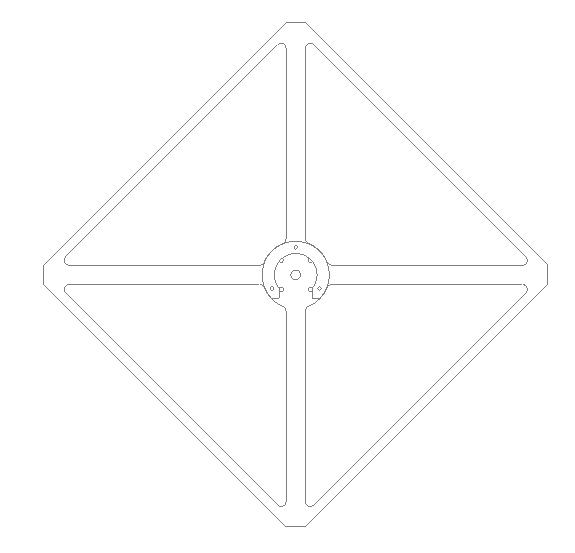
\includegraphics[scale=1]{graphics/cadfront.png}
  \caption{UAV frame front}
  \label{fig:CADfront}
\end{figure}


\begin{figure}[H]
  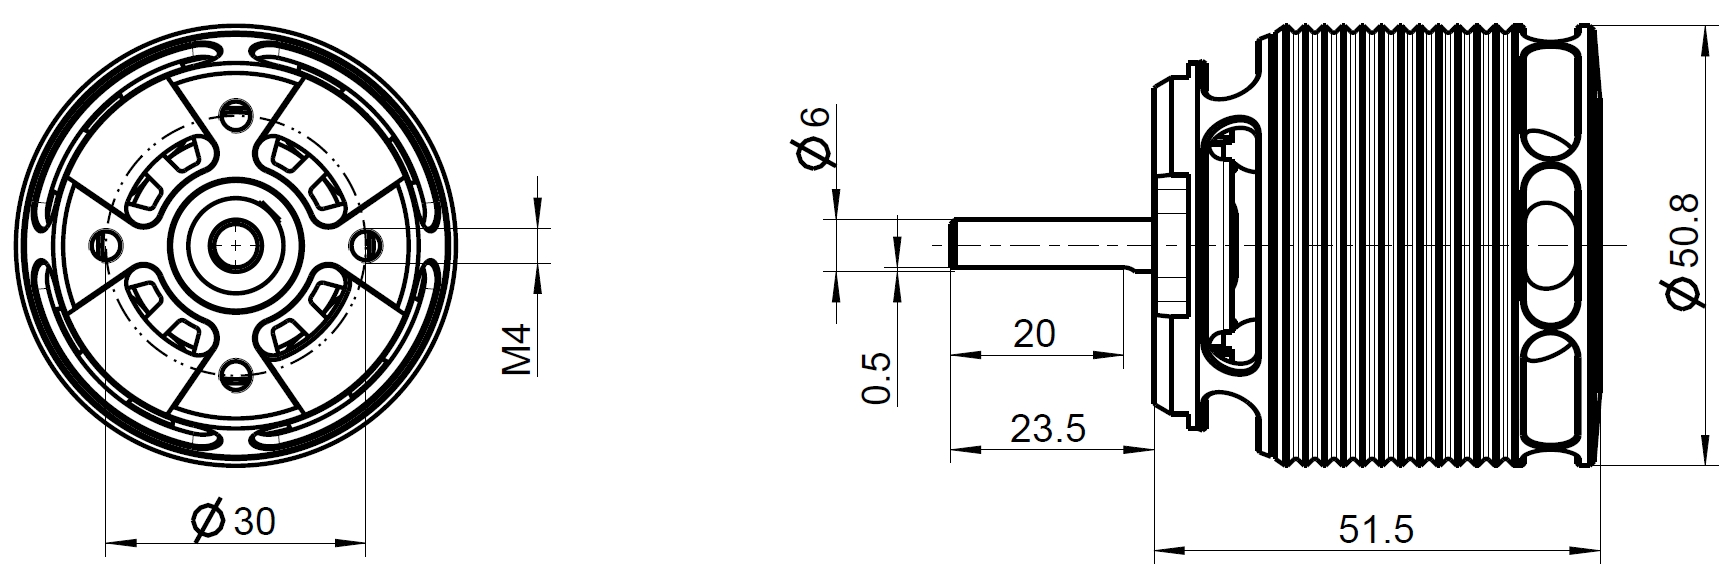
\includegraphics[scale=0.25]{graphics/Motor.jpg}
  \caption{Propeller Motor}
  \label{fig:Propeller Motor}
\end{figure}

\subsection{Graphs}

Median filter effect on IMU data

\begin{figure}[H]
  \centering
  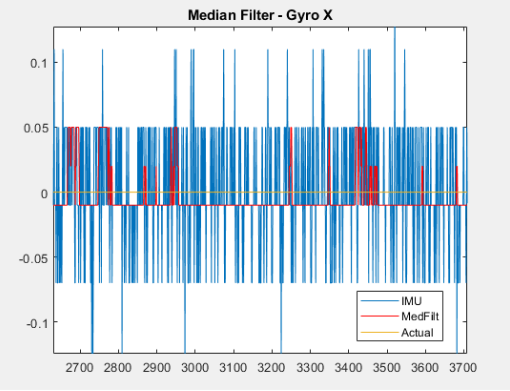
\includegraphics[scale=0.8]{graphics/median.png}
  \caption{Median filter effects on data}
  \label{fig:Median Filter}
\end{figure}


\begin{figure}[H]
    \centering
    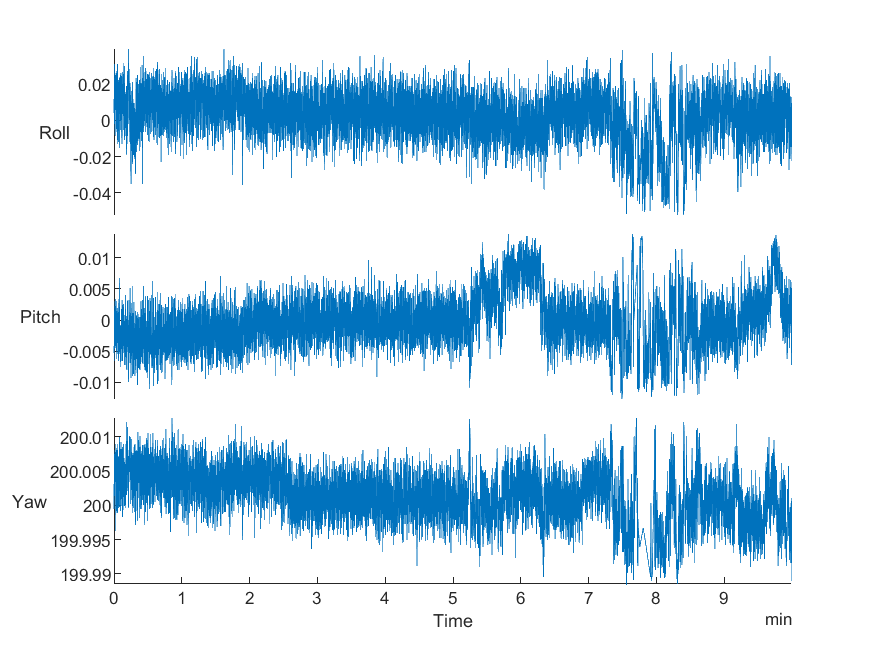
\includegraphics[scale=1]{graphics/Navigation/StackedStaticOpti.png}
    \caption{Stacked axes of reference Optitrack signal for static test}
     \label{fig:Stacked axes of reference Optitrack signal for static test}
\end{figure} 


\begin{figure}[H]
    \centering
    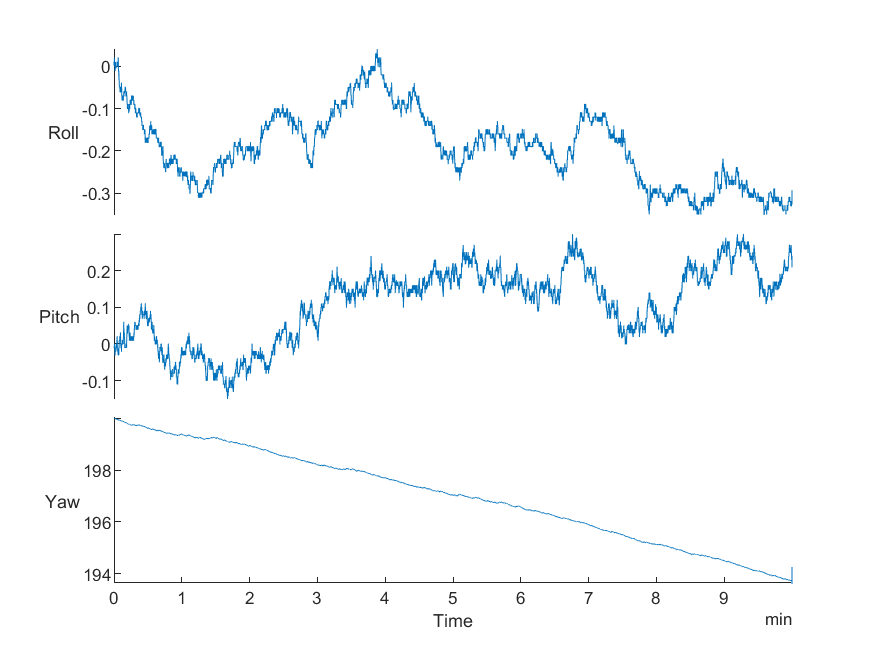
\includegraphics[scale=1]{graphics/Navigation/StackedStaticGyro.png}
    \caption{Stacked axes of integrated gyro signal for static test}
     \label{fig:Stacked axes of integrated gyro signal for static test}
\end{figure}

\begin{figure}[H]
    \centering
    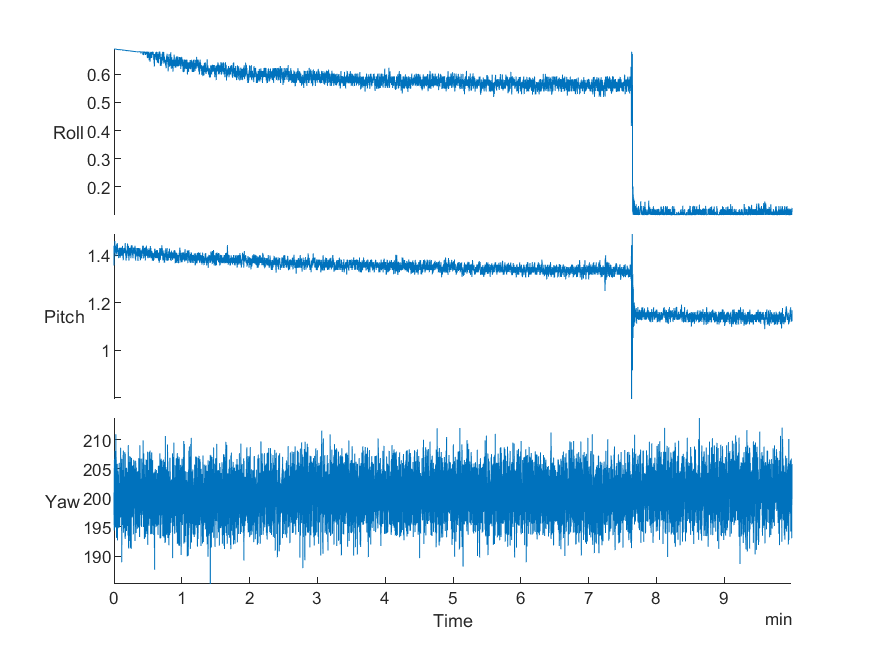
\includegraphics[scale=1]{graphics/Navigation/StackedStaticComp.png}
    \caption{Stacked axes of complementary filter signal for static test}
     \label{fig:Stacked axes of complementary filter signal for static test}
\end{figure}

\begin{figure}[H]
    \centering
    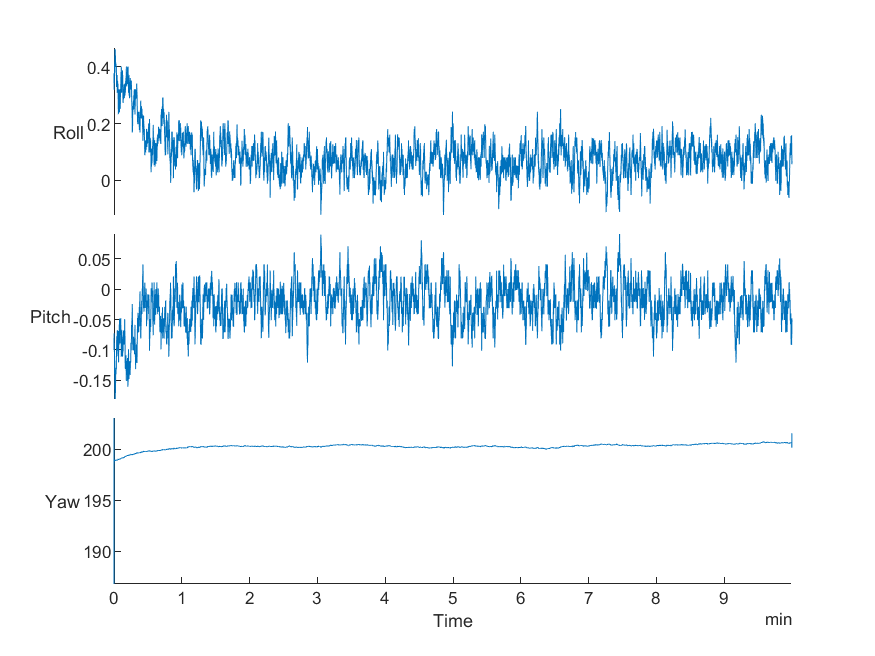
\includegraphics[scale=1]{graphics/Navigation/StackedStaticMahony.png}
    \caption{Stacked axes of Mahony filter signal for static test}
     \label{fig:Stacked axes of Mahony filter signal for static test}
\end{figure}

\begin{figure}[H]
    \centering
    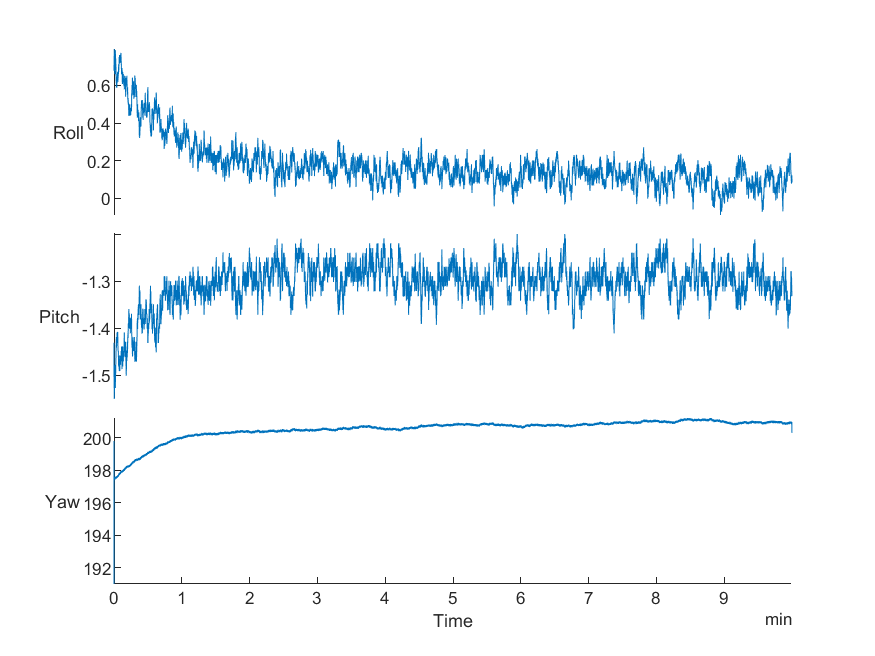
\includegraphics[scale=1]{graphics/Navigation/StackedStaticMadgwick.png}
    \caption{Stacked axes of Madgwick filter signal for static test}
     \label{fig:Stacked axes of Madgwick filter signal for static test}
\end{figure}


\begin{figure}[H]
    \centering
    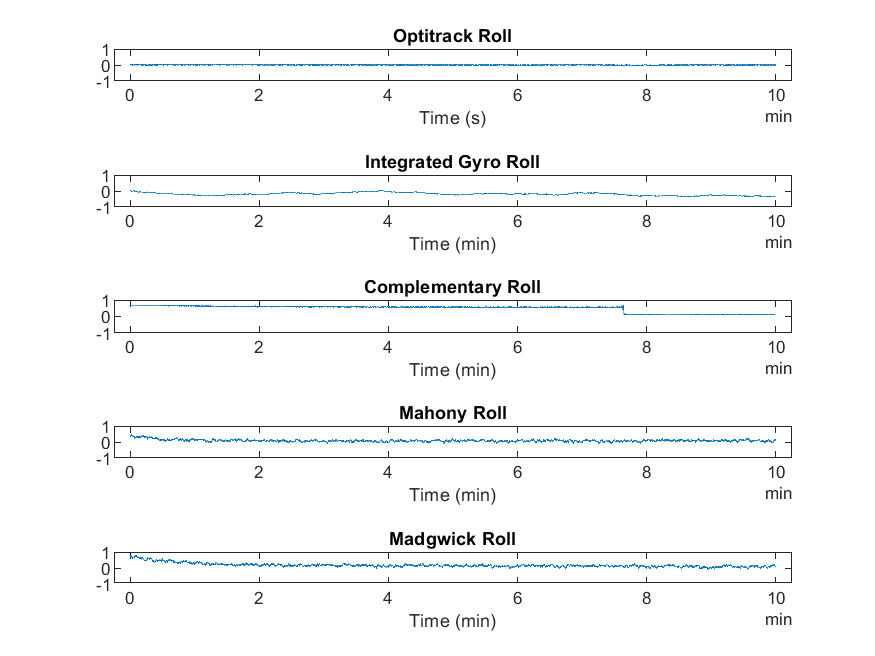
\includegraphics[scale=1]{graphics/Navigation/TiledStaticRoll.png}
    \caption{Tiled plot of roll axes for static test}
     \label{fig:Tiled plot of filters roll axes for static test}
\end{figure}

\begin{figure}[H]
    \centering
    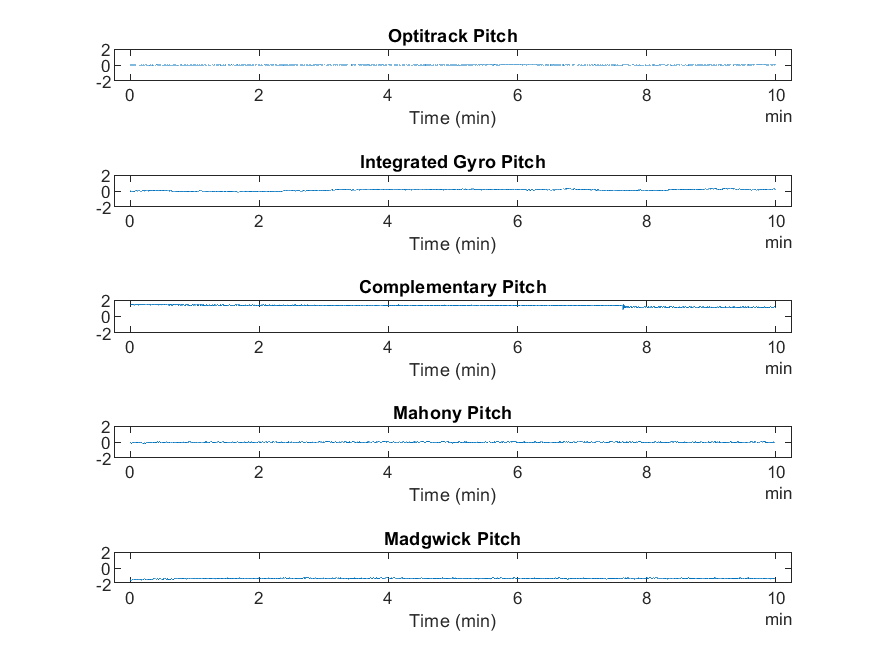
\includegraphics[scale=1]{graphics/Navigation/TiledStaticPitch.png}
    \caption{Tiled plot of pitch axes for static test}
     \label{fig:Tiled plot of filters pitch axes for static test}
\end{figure}

\begin{figure}[H]
    \centering
    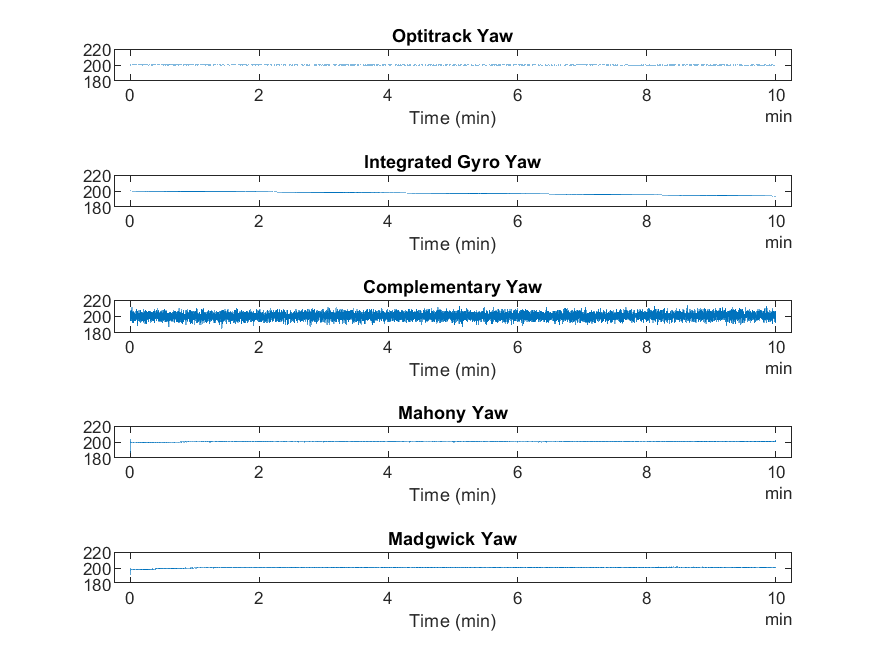
\includegraphics[scale=1]{graphics/Navigation/TiledStaticYaw.png}
    \caption{Tiled plot of yaw axes for static test}
     \label{fig:Tiled plot of filters yaw axes for static test}
\end{figure}

Static navigation tests: combined plots

\begin{figure}[H]
    \centering
    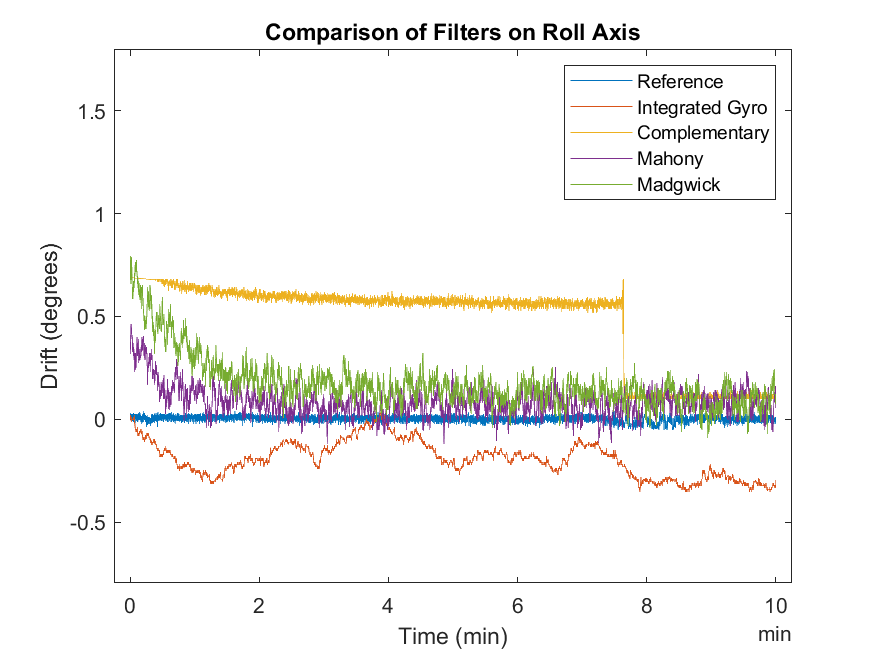
\includegraphics[scale=1]{graphics/Navigation/CombinedStaticRoll.png}
    \caption{Combined plot of roll axes for static test}
     \label{fig:Combined plot of roll axes for static test}
\end{figure}


\begin{figure}[H]
    \centering
    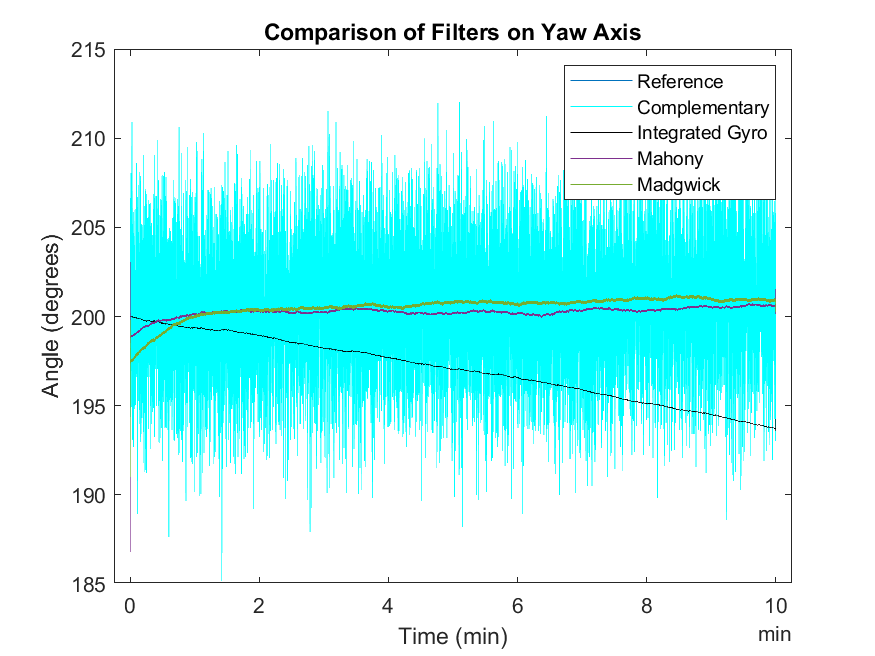
\includegraphics[scale=1]{graphics/Navigation/CombinedStaticYaw.png}
    \caption{Combined plot of yaw axes for static test}
     \label{fig:Combined plot of yaw axes for static test}
\end{figure}


\begin{figure}[H]
    \centering
    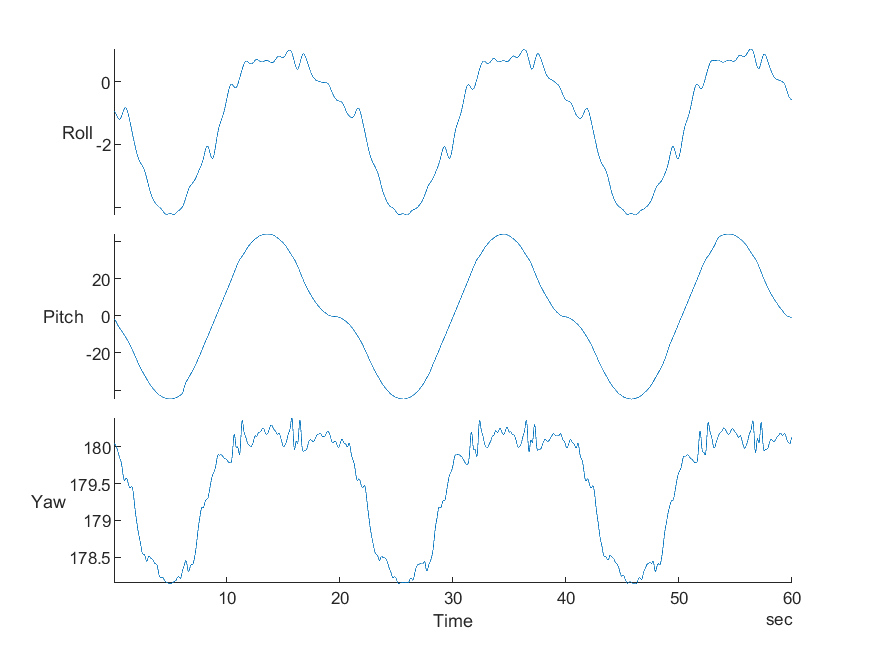
\includegraphics[scale=1]{graphics/Navigation/StackedMotionOpti.png}
    \caption{Stacked axes of reference Optitrack signal for motion test}
     \label{fig:Stacked axes of reference Optitrack signal for motion test}
\end{figure} 


\begin{figure}[H]
    \centering
    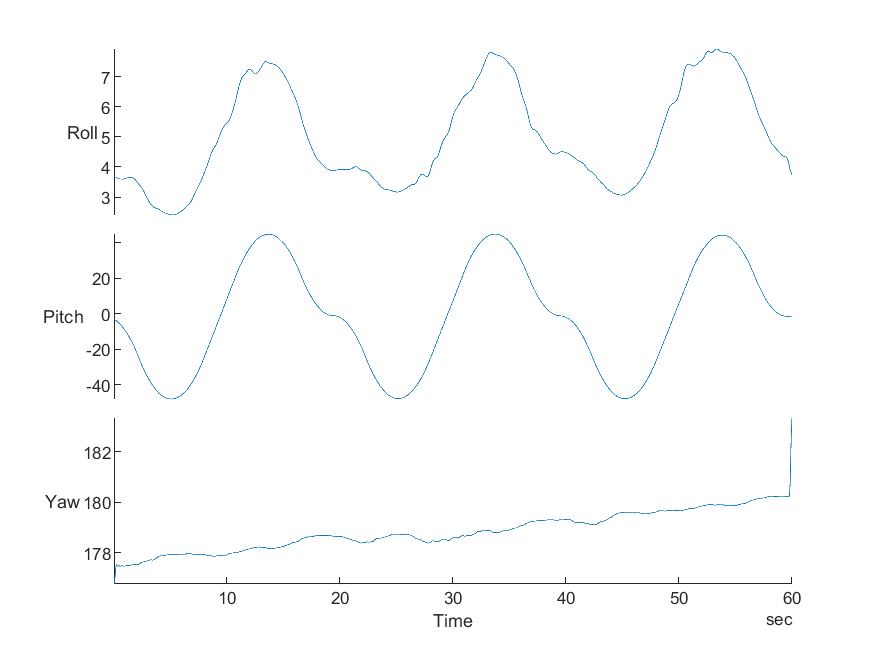
\includegraphics[scale=1]{graphics/Navigation/StackedMotionGyro.png}
    \caption{Stacked axes of integrated gyro signal for motion test}
     \label{fig:Stacked axes of integrated gyro signal for motion test}
\end{figure}

\begin{figure}[H]
    \centering
    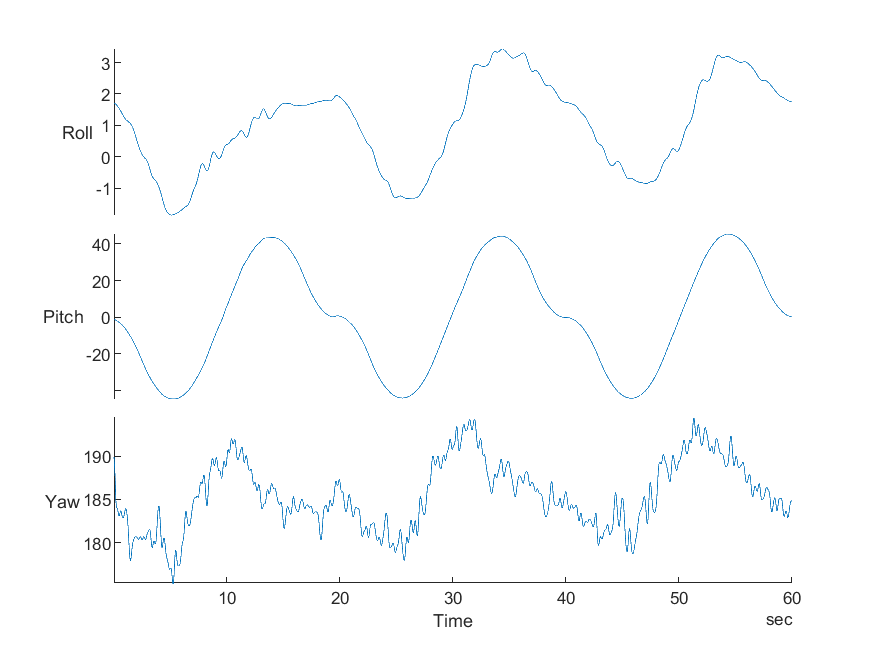
\includegraphics[scale=1]{graphics/Navigation/StackedMotionComp.png}
    \caption{Stacked axes of complementary filter signal for motion test}
     \label{fig:Stacked axes of complementary filter signal for motion test}
\end{figure}

\begin{figure}[H]
    \centering
    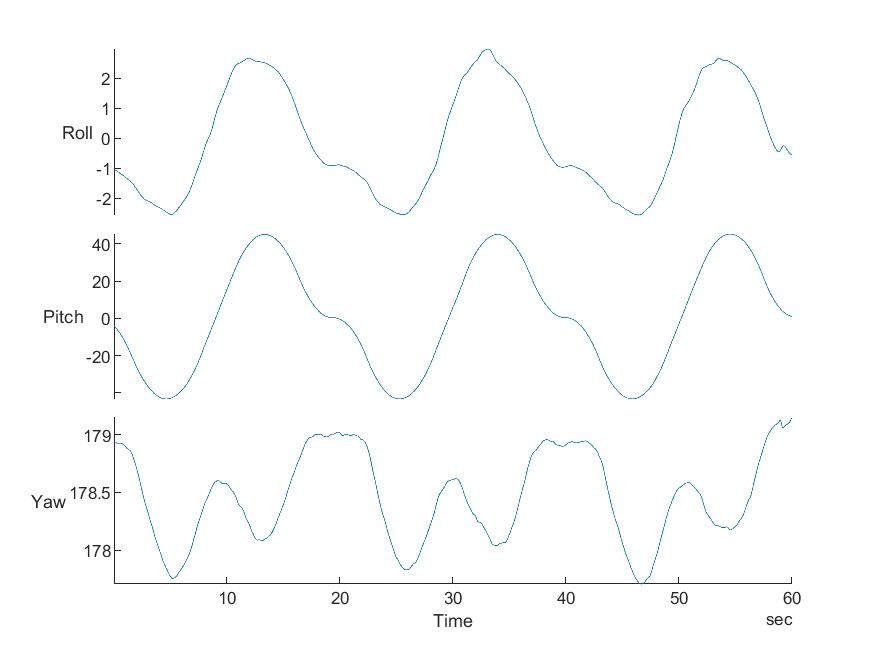
\includegraphics[scale=1]{graphics/Navigation/StackedMotionMahony.png}
    \caption{Stacked axes of Mahony filter signal for motion test}
     \label{fig:Stacked axes of Mahony filter signal for motion test}
\end{figure}

\begin{figure}[H]
    \centering
    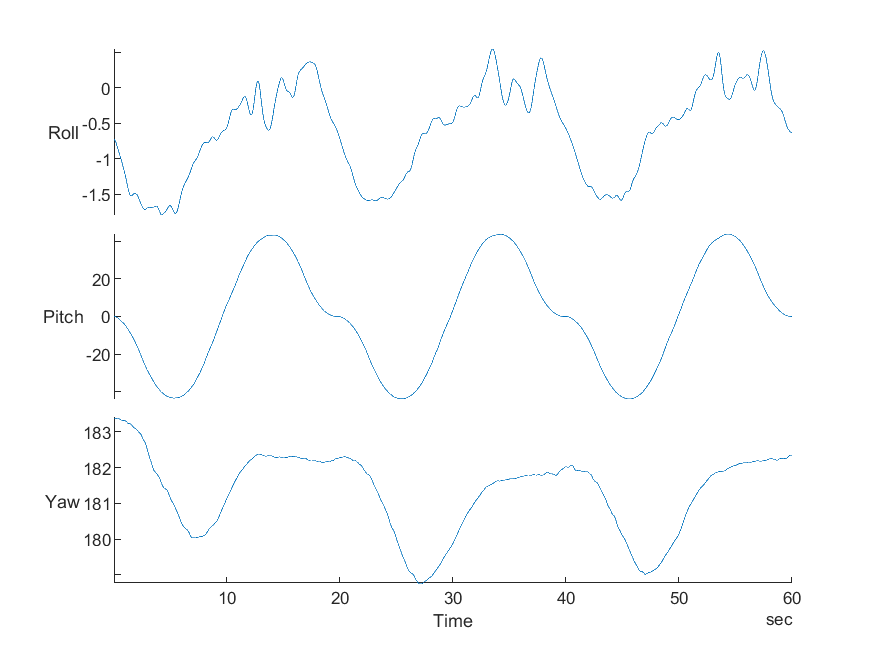
\includegraphics[scale=1]{graphics/Navigation/StackedMotionMadgwick.png}
    \caption{Stacked axes of Madgwick filter signal for motion test}
     \label{fig:Stacked axes of Madgwick filter signal for motion test}
\end{figure}


\begin{figure}[H]
    \centering
    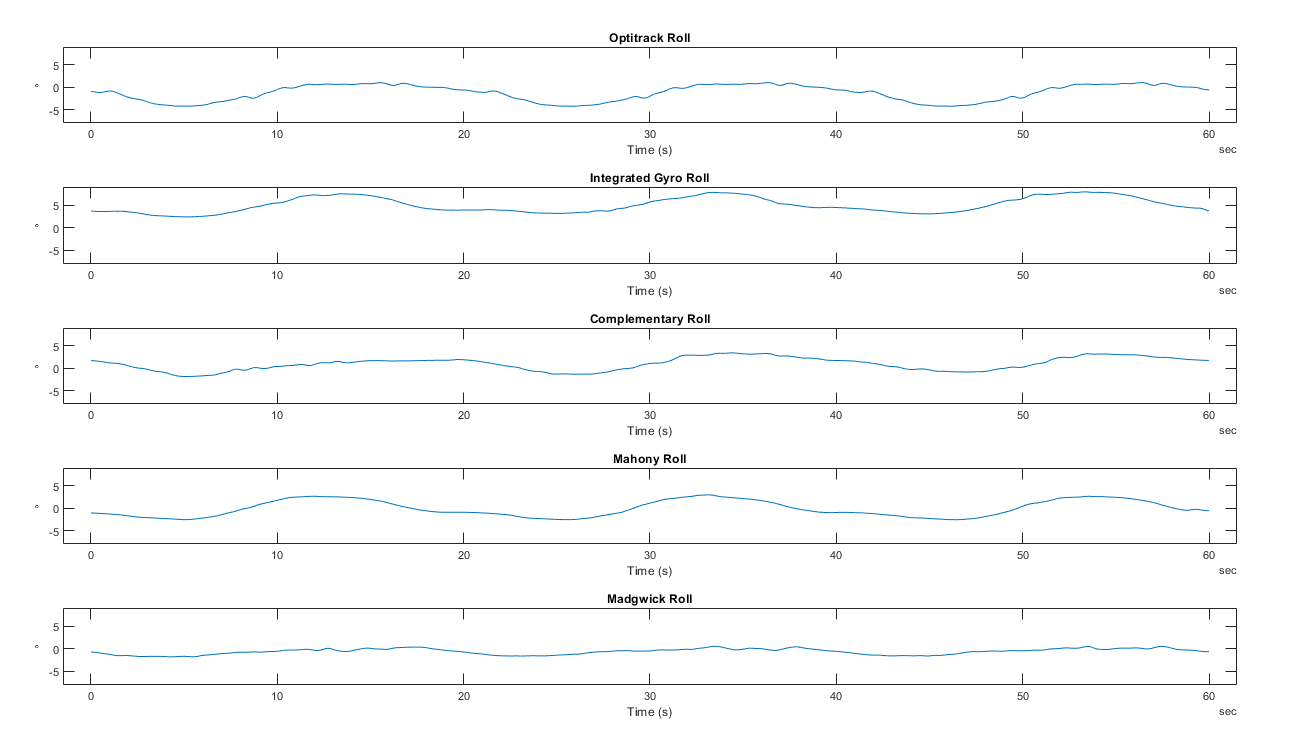
\includegraphics[scale=0.5]{graphics/Navigation/TiledMotionRoll.png}
    \caption{Tiled plot of roll axes for motion test}
     \label{fig:Tiled plot of filters roll axes for motion test}
\end{figure}

\begin{figure}[H]
    \centering
    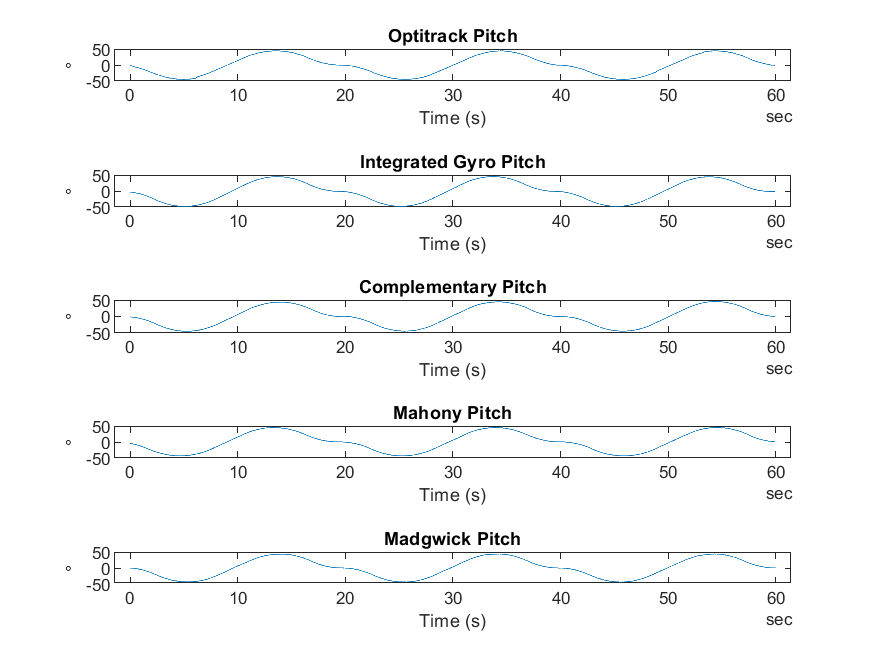
\includegraphics[scale=1]{graphics/Navigation/TiledMotionPitch.png}
    \caption{Tiled plot of pitch axes for motion test}
     \label{fig:Tiled plot of filters pitch axes for motion test}
\end{figure}

\begin{figure}[H]
    \centering
    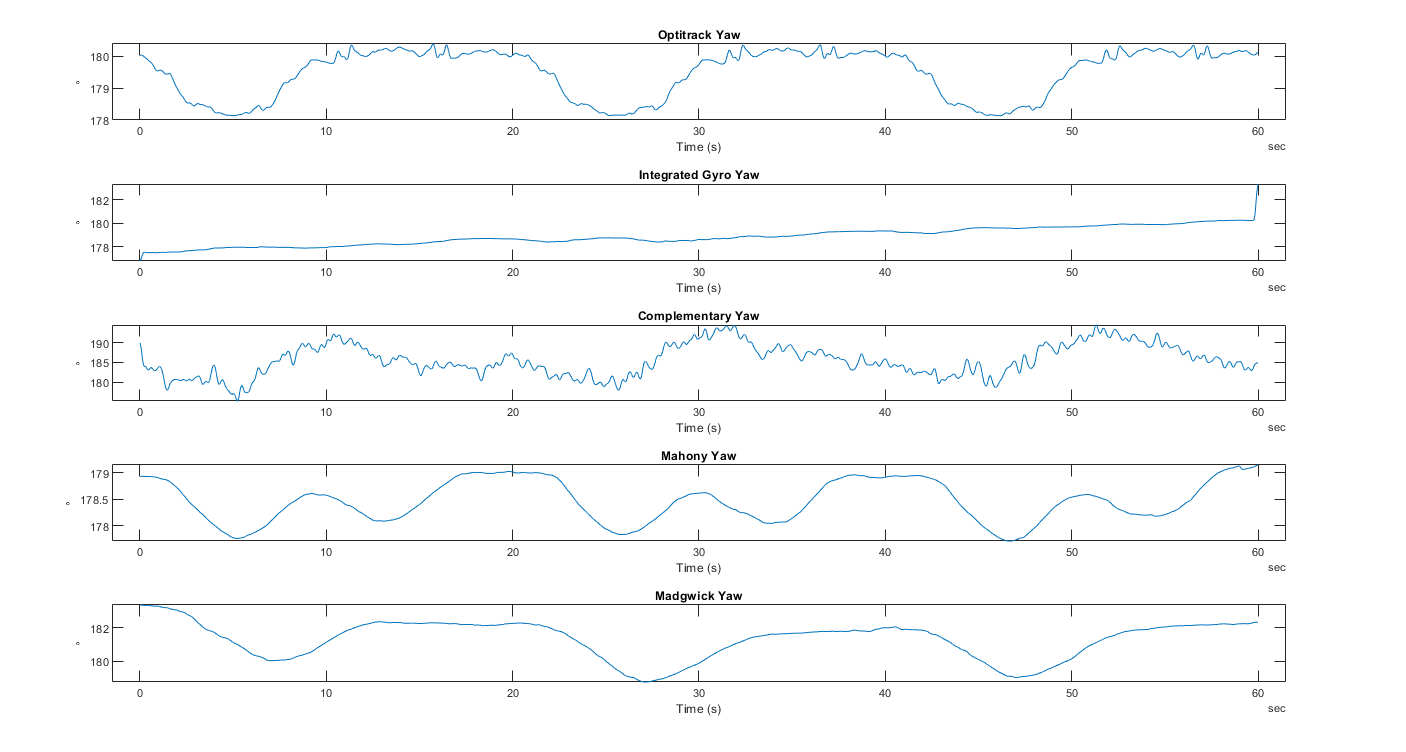
\includegraphics[scale=0.5]{graphics/Navigation/TiledMotionYaw.png}
    \caption{Tiled plot of yaw axes for motion test}
     \label{fig:Tiled plot of filters yaw axes for motion test}
\end{figure}


\begin{figure}[H]
    \centering
    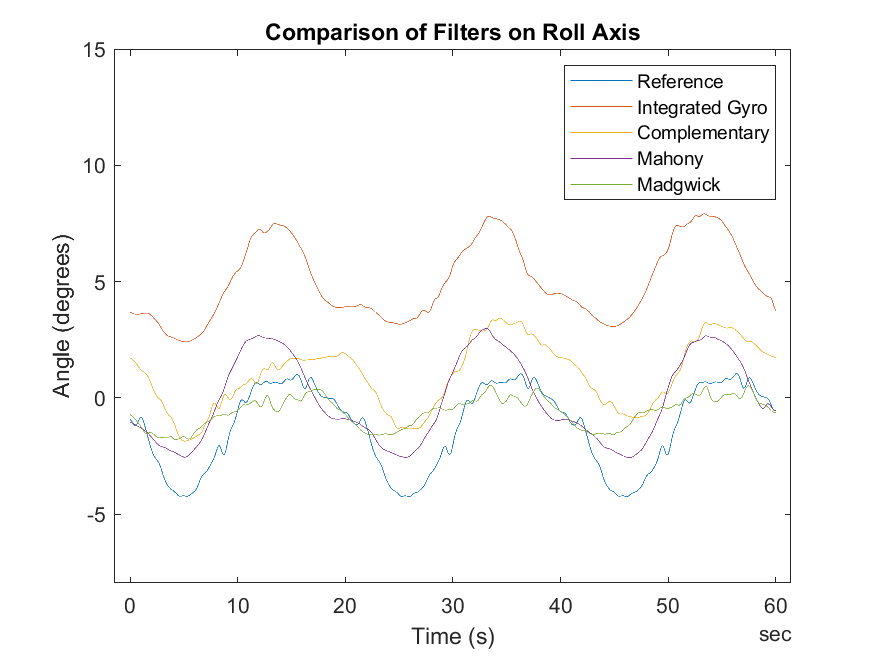
\includegraphics[scale=1]{graphics/Navigation/CombinedMotionRoll.png}
    \caption{Combined plot of roll axes for motion test}
     \label{fig:Combined plot of roll axes for motion test}
\end{figure}


\begin{figure}[H]
    \centering
    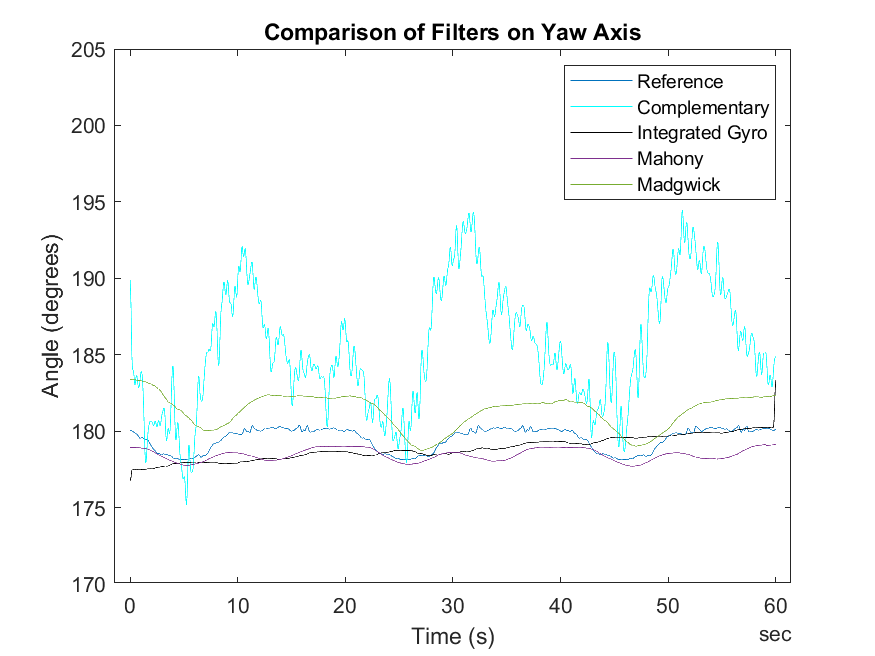
\includegraphics[scale=1]{graphics/Navigation/CombinedMotionYaw.png}
    \caption{Combined plot of yaw axes for motion test}
     \label{fig:Combined plot of yaw axes for motion test}
\end{figure}

\subsection{Model Validation}


\begin{figure}[H]
  \centering
  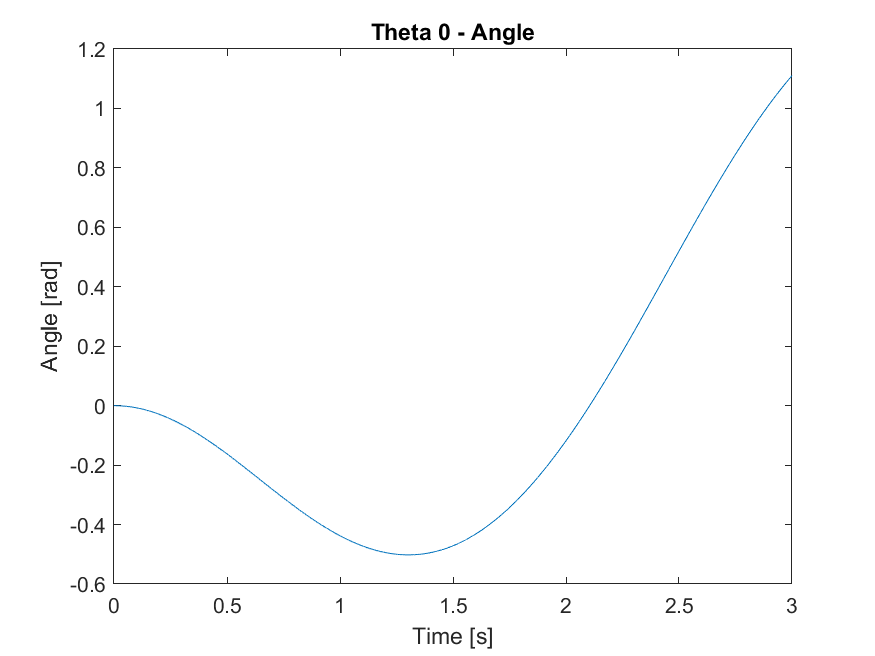
\includegraphics[scale=1]{graphics/Integration/theta0.png}
  \caption{Model validation applied forces: body 0 angle}
  \label{fig:Model validation applied forces: body 0 angular position}
\end{figure}


\begin{figure}[H]
  \centering
  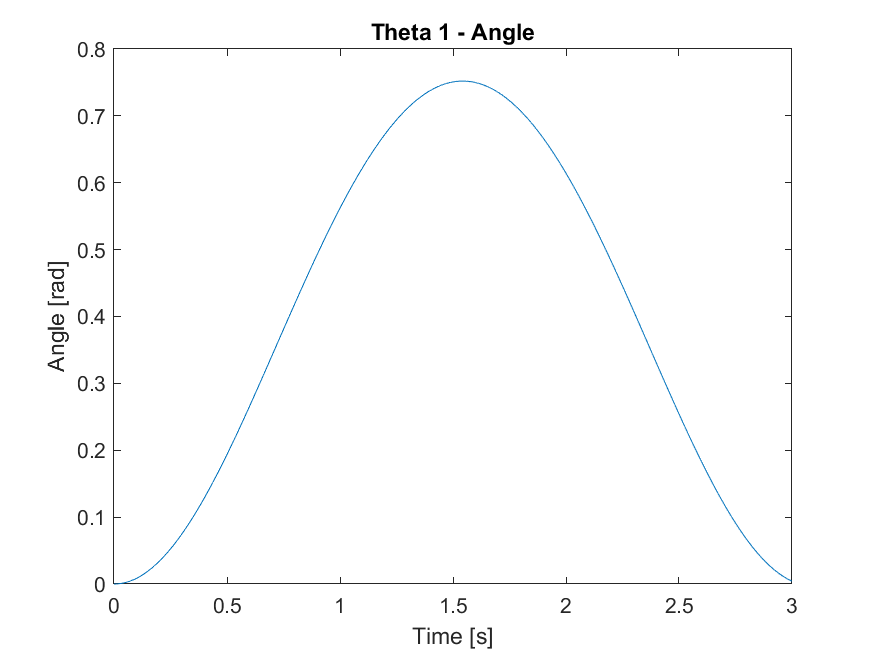
\includegraphics[scale=1]{graphics/Integration/theta1.png}
  \caption{Model validation applied forces: body 1 angle}
  \label{fig:Model validation applied forces: body 1 angular position}
\end{figure}

\begin{figure}[H]
  \centering
  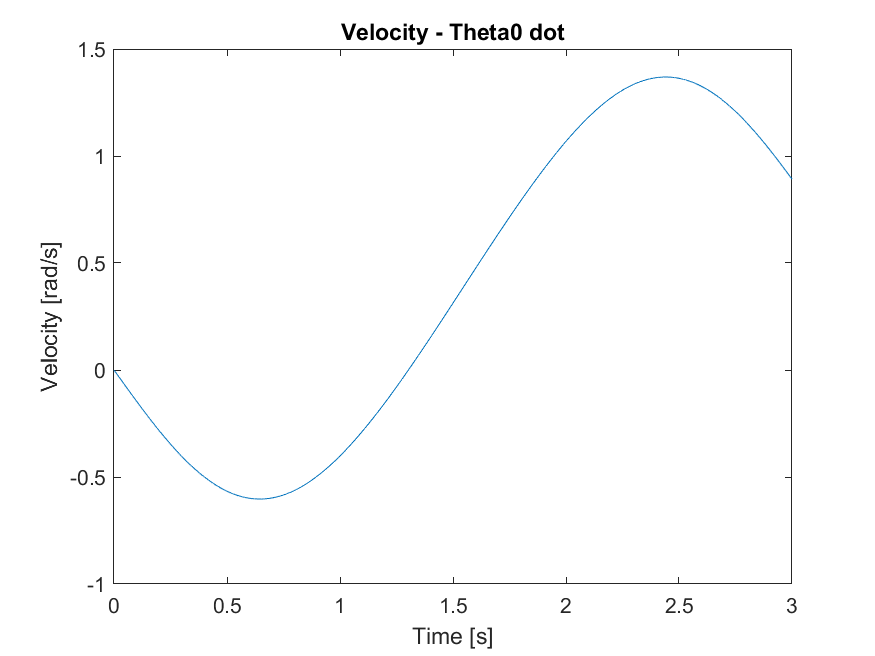
\includegraphics[scale=1]{graphics/Integration/dtheta0.png}
  \caption{Model validation applied forces: body 0}
  \label{fig:Model validation applied forces: body 0 velocity}
\end{figure}

Control: tuning process

\begin{figure}[H]
  \centering
  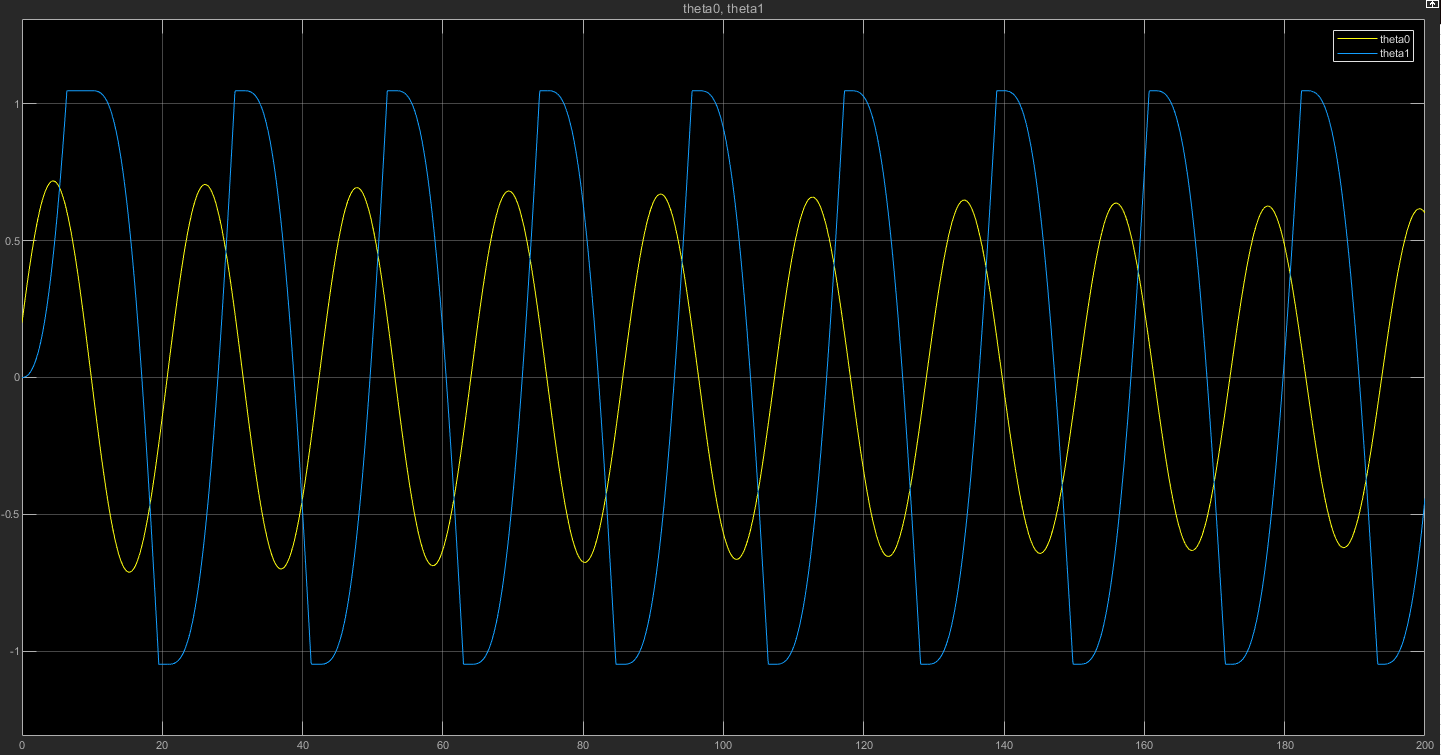
\includegraphics[scale=0.4]{graphics/Control/P0.5.png}
  \caption{Controller tuning process: kP=0.5}
  \label{fig:Controller tuning process: kP=0.5}
\end{figure}

\begin{figure}[H]
  \centering
  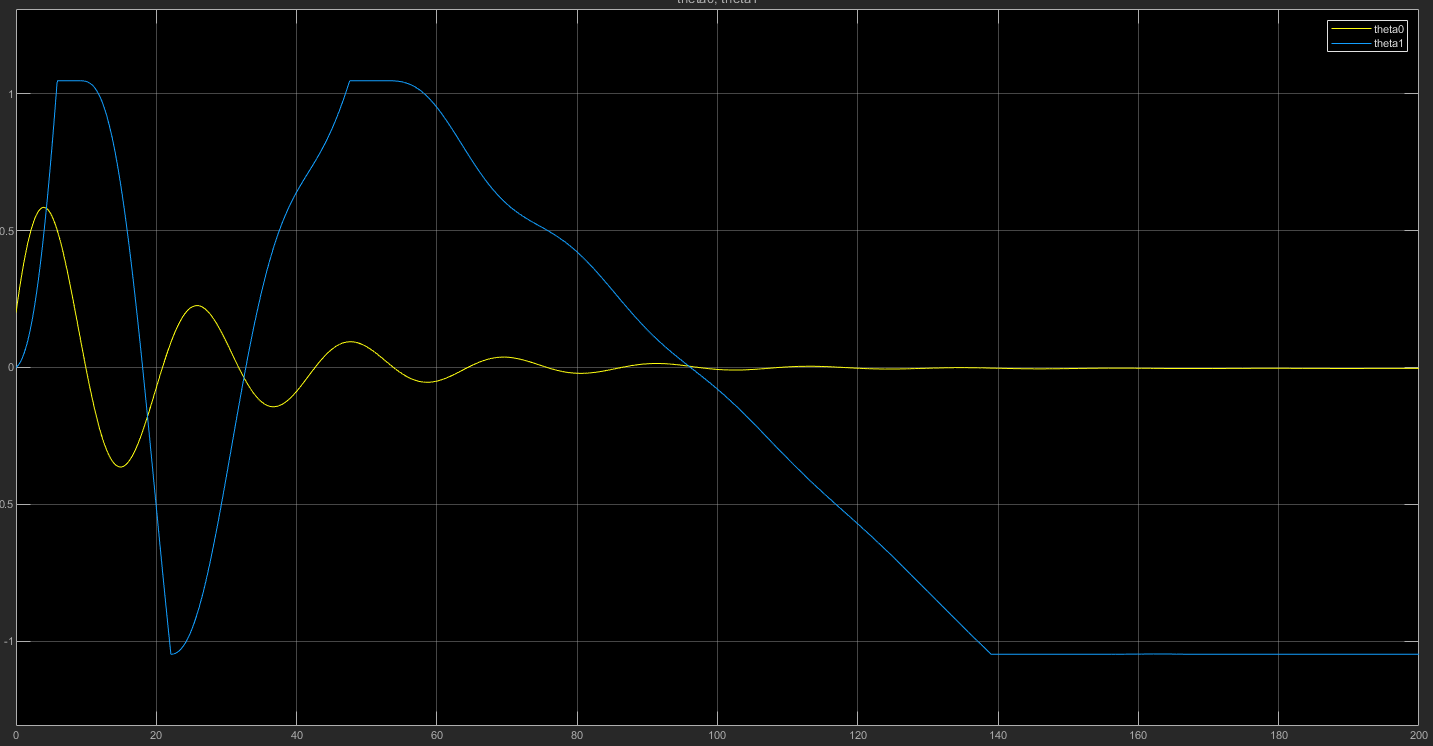
\includegraphics[scale=0.4]{graphics/Control/P0.5,D0.5.png}
  \caption{Controller tuning process: kP=0.5, kD=0.5}
  \label{fig:Controller tuning process: kP=0.5, kD=0.5}
\end{figure}


\begin{figure}[H]
  \centering
  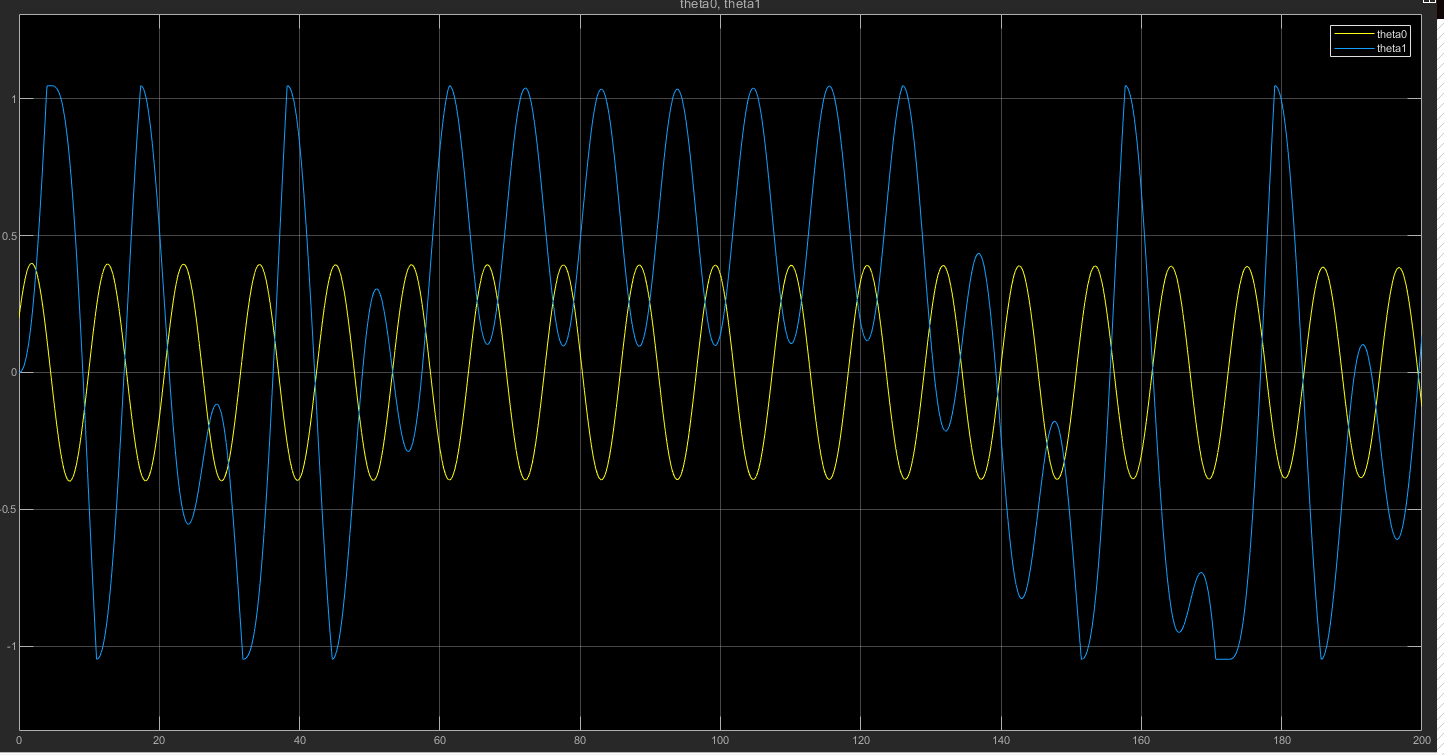
\includegraphics[scale=0.4]{graphics/Control/p2.png}
  \caption{Controller tuning process: kP2}
  \label{fig:Controller tuning process: kP=2}
\end{figure}
